%!TEX program = pdflatex
\documentclass[12pt,a4paper,oneside]{report}

% ============================================================
% PACKAGES
% ============================================================
\usepackage[utf8]{inputenc}
\usepackage[T1]{fontenc}
\usepackage{geometry}
\geometry{
    a4paper,
    left=3cm,
    right=3cm,
    top=2.5cm,
    bottom=2.5cm
}
\usepackage{pdfpages}
\usepackage{hyperref}
\hypersetup{
    colorlinks=true,
    linkcolor=black,
    citecolor=black,
    urlcolor=blue,
    pdftitle={The Meta-Learning Gap: Combining Hydra and Quant for Large-Scale Time Series Classification},
    pdfauthor={Urav Maniar},
    pdfsubject={Master of Data Science Thesis},
    pdfkeywords={time series classification, ensemble methods, meta-learning}
}
\usepackage{microtype}
\usepackage{setspace}
\onehalfspacing

% ============================================================
% DOCUMENT
% ============================================================
\begin{document}

% ============================================================
% COVER PAGE
% ============================================================
\begin{titlepage}
\centering
\vspace*{1.5cm}

{\LARGE\bfseries Monash University}\\[0.5cm]
{\large Faculty of Information Technology}\\[2cm]

{\Huge\bfseries The Meta-Learning Gap:\\[0.4cm]
Combining Hydra and Quant for\\[0.4cm]
Large-Scale Time Series Classification}\\[2cm]

{\Large Urav Maniar}\\[0.4cm]
{\large Student ID: 30071461}\\[0.2cm]
{\large Supervisor: Angus Dempster}\\[2cm]

{\large A thesis submitted in partial fulfilment of the requirements\\[0.3cm]
for the degree of}\\[0.5cm]
{\large\bfseries Master of Data Science}\\[1.5cm]

{\large \today}

\vfill

\end{titlepage}

% ============================================================
% TABLE OF CONTENTS
% ============================================================
\tableofcontents
\clearpage

% ============================================================
% PART 1: LITERATURE REVIEW AND Project PROPOSAL
% ============================================================
\part{Literature Review and Project Proposal}

% Include Literature Review PDF
% Note: pagecommand={\thispagestyle{empty}} removes page numbers from included pages
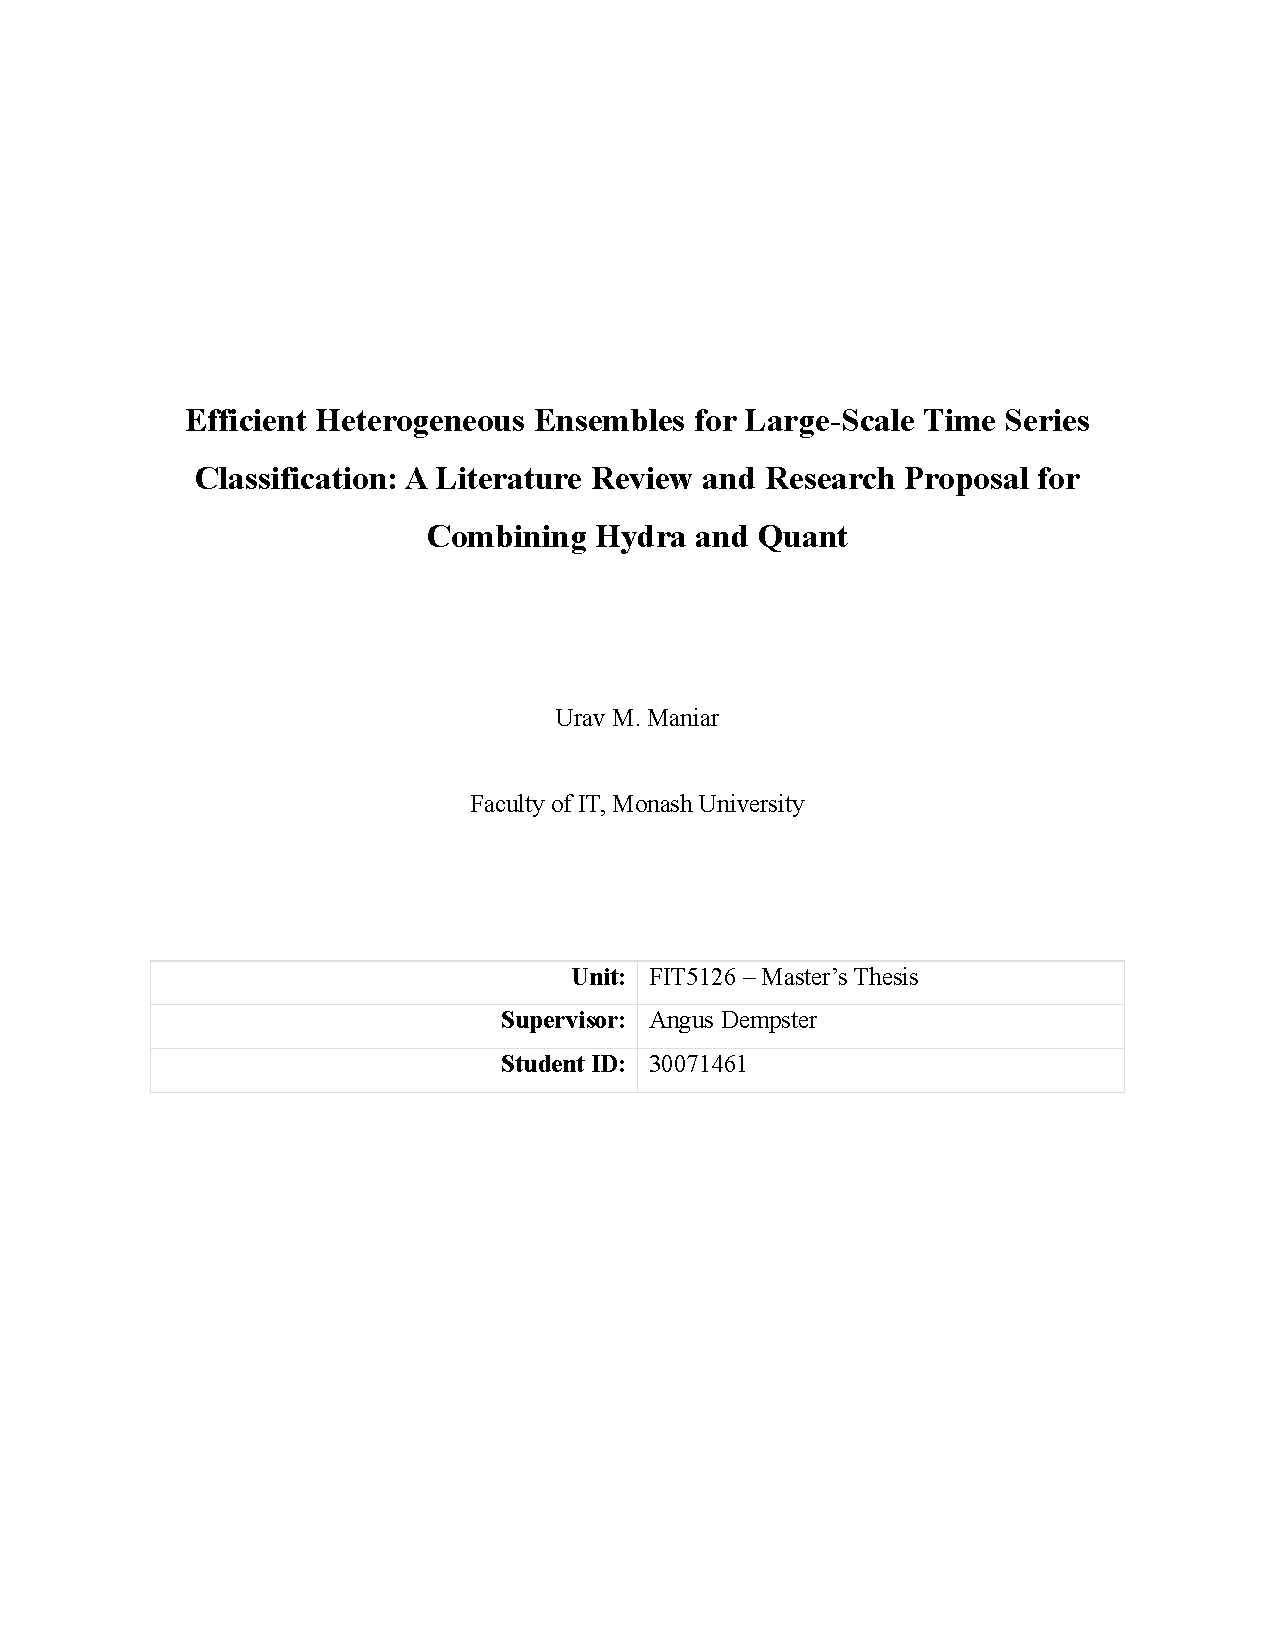
\includepdf[
    pages=-,
    pagecommand={\thispagestyle{empty}}
]{literature-review.pdf}

% ============================================================
% PART 2: RESEARCH PAPER (INCLUDING APPENDICES)
% ============================================================
\part{Research Paper (including Appendices)}

% Include Research Paper PDF
% Note: The appendices are contained within this document, appearing after
% the references section as per standard academic paper format.
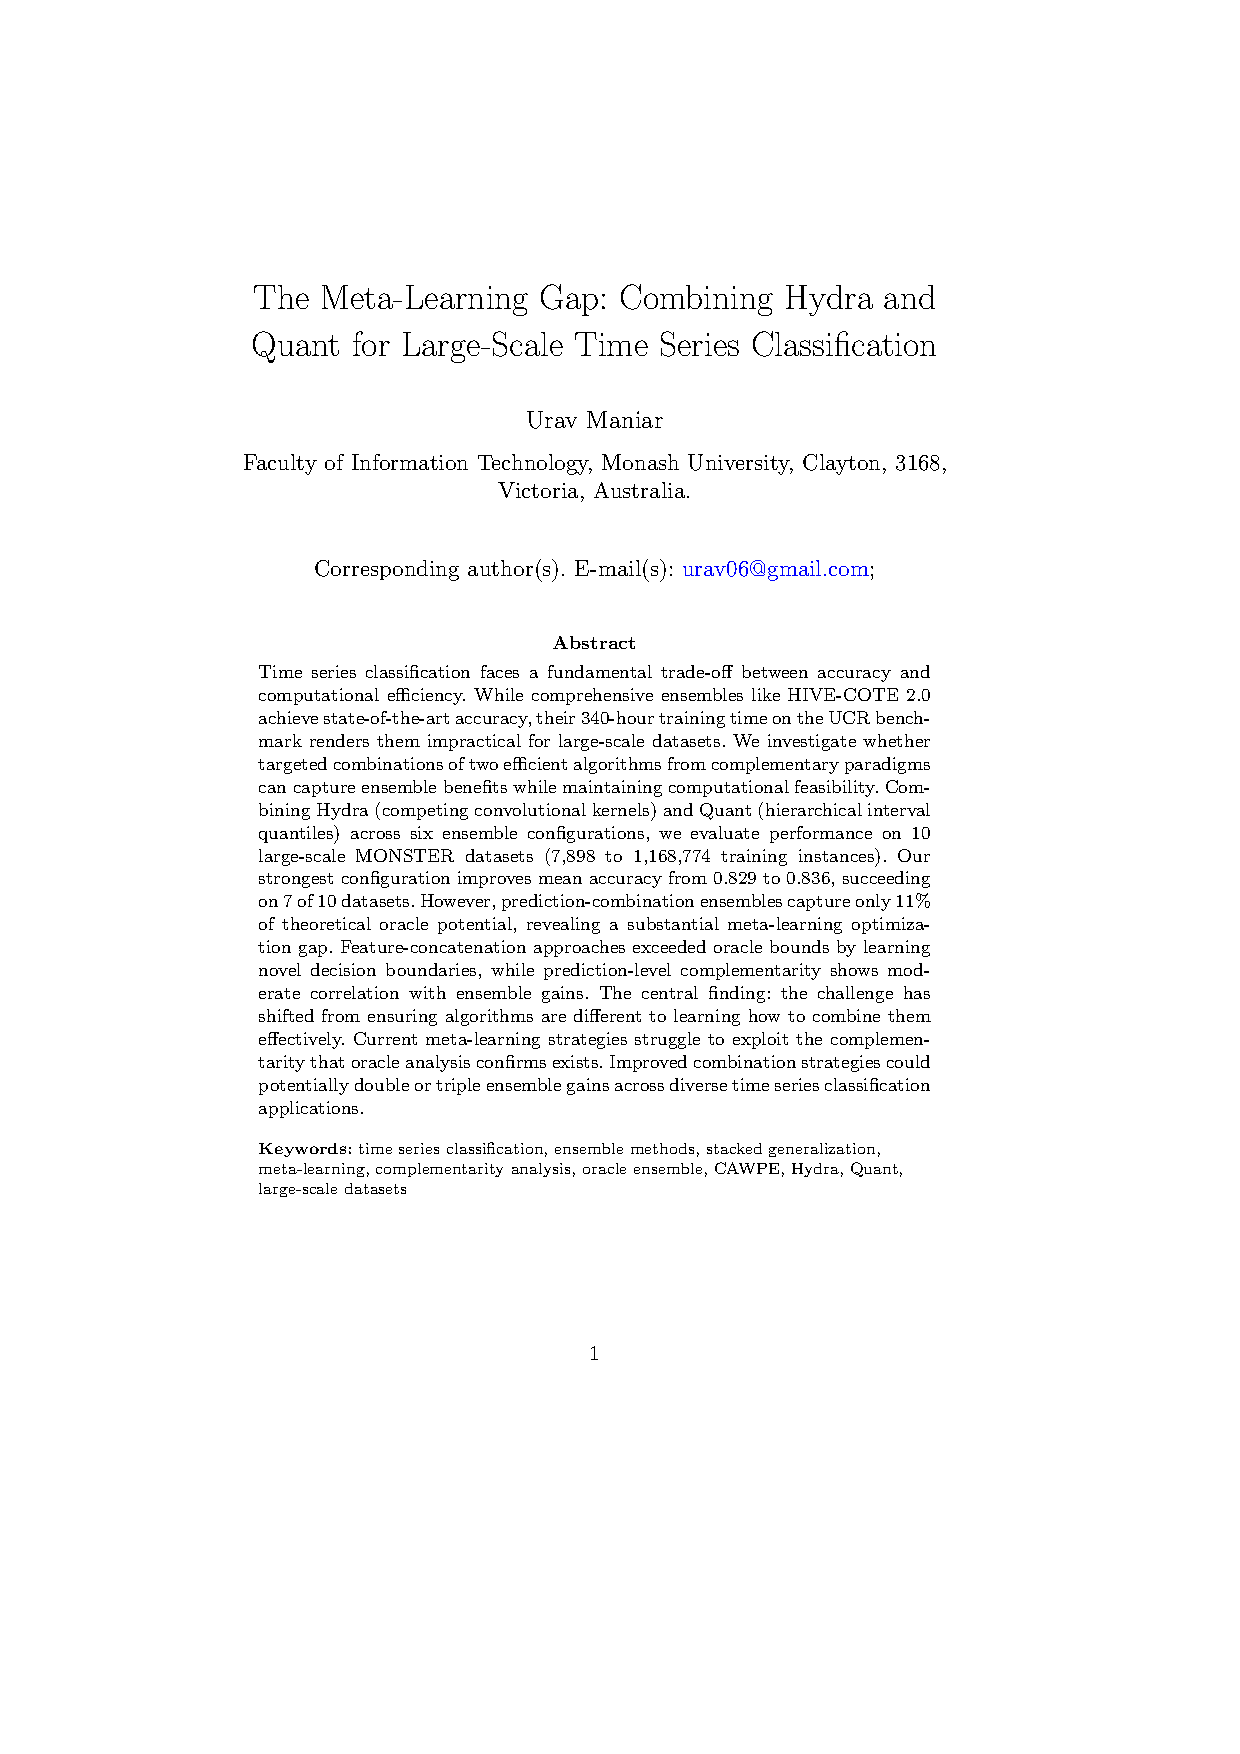
\includepdf[
    pages=-,
    pagecommand={\thispagestyle{empty}}
]{research-paper.pdf}

\end{document}
